\documentclass[a4paper,12pt]{article}
\usepackage{pdfpages}
\usepackage{changepage}
\usepackage[french]{babel}
\usepackage[T1]{fontenc}
\usepackage[utf8]{inputenc}
\usepackage{enumitem}
\usepackage{helvet}
\usepackage{CormorantGaramond}
\usepackage{courier}
\usepackage{pifont}
\usepackage{microtype}
\usepackage{hyperref}
\usepackage{amsmath}
\usepackage{amssymb}
\usepackage{physics}
\usepackage{geometry}
\usepackage{stmaryrd}
\usepackage{color}
\usepackage{float}
\usepackage{graphicx} % Insérer des images
\usepackage[font=footnotesize,labelfont=bf]{caption}
\usepackage{subcaption}
\usepackage{mwe}
\usepackage{hyperref} % Créer des liens et des signets
\hypersetup{
colorlinks=true, %colorise les liens
breaklinks=true, %permet le retour à la ligne dans les liens trop longs
urlcolor= magenta, %couleur des hyperliens
linkcolor= cyan, %couleur des liens internes
citecolor=green, %couleur des références
pdftitle={MLPAP24_SR_3_IR}, %informations apparaissant dans
pdfauthor={3}, %les informations du document
pdfsubject={MLPAP24_SR_3_IR} %sous Acrobat.
}
\geometry{hmargin=1.5cm,vmargin=1.6cm}

\newcommand{\parallelsum}{\mathbin{\!/\mkern-5mu/\!}}
%\newcommand{\mathrm}{\mathrm}

\setlength\parindent{0pt}

\title{Projet \emph{Machine Learning}\\Régression symbolique -- Groupe 3}
\author{}
\date{}

\begin{document}

\colorlet{mygreen}{green!45!black}

\newenvironment{myfont}{\scriptsize\fontfamily{phv}\selectfont}{\par}

\newcommand{\nicolas}[1]{\textcolor{blue}{[Nicolas : #1]}}

\maketitle

\noindent\fbox{\parbox{\textwidth}{
\begin{myfont}
Une coloration indique l'état d'avancement des différentes propositions avancées : \\
{\color{mygreen} fait} ; \\
{\color{orange} en cours} ; \\
{\color{red} prévu, confiance dans la méthode à mettre en œuvre} ; \\
{\color{blue} aucune idée de la méthode à mettre en œuvre/doute sur la pertinence de la proposition} ; \\
sans objet
\end{myfont}
}}

\section{Contexte}

\subsection{Position du problème : la régression symbolique}

Supposons que l'on dispose -- par exemple à la suite de l'étude expérimentale d'un système physique quelconque -- d'un jeu de variables ${(x_1, x_2, ..., x_n, y_1, ..., y_p)_j}$. On souhaite comprendre le fonctionnement de ce système sous la forme d'une ou plusieurs relations entre ces différentes variables. On peut, par exemple, vouloir exprimer les $p$ dernières variables  $(y_1, ..., y_p)$, regroupées dans la \emph{sortie} $\vb y \equiv \begin{pmatrix}
y_1 \\
... \\
y_p
\end{pmatrix}$, selon les $n$ premières, qui forme les éléments de l'\emph{entrée} $\vb x \equiv \begin{pmatrix}
x_1 \\
... \\
x_n
\end{pmatrix}$ :

\[
\vb y = f(\vb x)
\]

Il se peut que nous ignorions tout de la physique du système, et que nous espérions que le jeu de données nous informe sur la forme de la fonction $f$ qui la contient. On dira que l'on \emph{résout le problème} $(\vb x, \vb y)$ lorsque l'on détermine la forme de la fonction $f$ telle que, avec une précision $\epsilon$ satisfaisante, on peut écrire : 

\[
\vb y = f(\vb x) + \vb e, \norm{\vb e} \leq \epsilon.
\]

Dans la suite on ne s'intéressera qu'à des problèmes où $p = 1$, le cas $p>1$ pouvant être reformulé comme l'assemblage de $p$ problèmes à $p=1$ indépendants.

\subsection{Implémentation et pertinence du \emph{machine learning}}

Moyennant de bonnes représentations, autant pour les éléments $(\vb x, \vb y)$ que pour la fonction $f$ les reliant, on peut espérer entraîner un modèle à retrouver l'expression de $f$ dans un jeu de données d'entraînement de la forme $\{(\vb x, \vb y)_j\}$. Ce jeu de données devra être de caractéristiques similaires aux problèmes que l'on cherchera à résoudre.

Évidemment, pour que le résultat final soit exploitable pour un opérateur humain, il nous faudra spécifier la forme que pourra prendre la fonction $f$. Typiquement, celle-ci pourra composer, sommer, multiplier :

\begin{itemize}

\item les variables $(x_1, x_2, ..., x_n)$

\item des opérateurs unaires $\Gamma : u \mapsto v$ associant un vecteur à un vecteur.

\underline{Exemple :} l'opérateur opposé, noté $\mathrm{opp}$, renvoie l'opposé d'un nombre. L'opérateur cosinus, noté $\mathrm{cos}$, renvoie le cosinus d'un nombre.

\item des opérateurs binaires $\lambda : u, v \mapsto w$ associant un vecteur à une paire de vecteurs.

\underline{Exemple :} l'opérateur somme, noté $+$, renvoie la somme terme à terme de deux vecteurs de la même taille.

\item ...

\end{itemize}

\subsubsection{Représentation d'une expression algébrique sous forme d'un arbre}

\medskip
\noindent
\begin{minipage}{0.82\textwidth}
Les expressions mathématiques peuvent être représentées sous forme d'arbres, les opérateurs et les fonctions étant des nœuds internes, les opérandes comme enfants, et les nombres, constantes et variables comme feuilles. Un exemple ci-contre.

\subsubsection{Représentation machine du problème}

On pourra utiliser des architectures de type \texttt{seq2seq}, ie. prenant en entrée une liste $(x_1, x_2, ..., x_n, y)_j$ de \emph{variables d'entrée} et renvoyant sous la forme d'une liste l'expression de la fonction $f$. Convenant de l'arité des opérateurs utilisés et de règles de précédence, la notation préfixée (ou postfixée) permet d'exprimer de façon univoque un arbre sous la forme d'une séquence. L'expression prise en exemple est, sous forme de liste : $[+, *, 3, \text{pow}, x, 2, -, \cos, *, 2, x, 1]$.
\end{minipage}
\hfill
\begin{minipage}{=0.16\textwidth}
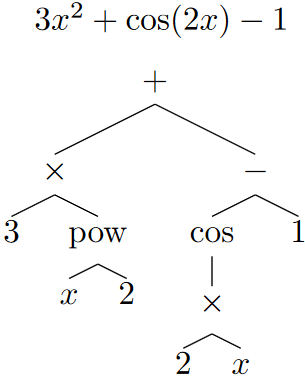
\includegraphics[width=\textwidth]{injectif.png}
\end{minipage}

\section{Fabrication d'un jeu de données}

Il s'est essentiellement agi d'implémenter la méthode décrite dans \cite{lample}.
On pourra également travailler en parallèle sur des jeux de données de référence, tels celui fabriqué dans \cite{udrescu}, ou ceux du \href{https://cavalab.org/srbench/}{SRbench}.

\subsection{Caractéristiques du jeu de données}
\label{sec:carac}

\subsubsection{{\color{orange}Pertinence}}
\label{sec:pert}

Dans la perspective d'utilisation du modèle pour résoudre des problèmes liés au monde réel, les expressions utilisées pour son entraînement devront être représentatives de celles susceptibles d'être rencontrées dans ses applications. Une grande diversité d'expressions ouvre plus de possibles mais au prix d'expressions bien plus lourdes à manipuler, et d'une durée d'assimilation croissant possiblement exponentiellement pour le modèle.

\begin{enumerate}

\item Taille $n$ du vecteur d'entrée\footnote{Pour une preuve de concept on pourra dans un premier temps le fixer à 1.}

\item Taille des arbres : borne supérieure sur le nombre de nœuds internes.

\item Structure des arbres. Faut-il, par exemple, qu'à nombre de noeuds donnés, l'arbre le plus \emph{left}(resp. \emph{right})\emph{-leaning}, le plus profond et le plus lage apparaissent avec la même probabilité ?

\item Quel jeu minimal d'opérateurs unaires et binaires employer ?

Vaut-il mieux introduire un opérateur $\text{opp}$ associant à une opérande son opposé, ou bien comprendre l'opposition comme une multiplication par -1 ? Considérer uniquement les lois de puissance entières les plus courantes (2 > 3), ou bien introduire un opérateur générique d'exponentiation, au risque de se retrouver avec des tas de solutions en $^{1.97}$ ?
\end{enumerate}

On pourra répondre à ces questions sur la base de jeux de référence tels que celui de \cite{udrescu}, ou ceux du \href{https://cavalab.org/srbench/}{SRbench}.

\subsubsection{{\color{blue}Représentativité}}
\label{sec:repr}

Ayant déterminé ses ingrédients (point précédent : la dimension $n$ du vecteur d'entrée, bornes sur le nombre de nœuds internes, fonctions utilisables, ...), trouver un moyen de déterminer quelle taille de jeu de données d'entraînement est suffisante pour rendre le modèle "performant" sur les problèmes susceptibles d'être rencontrés.

\medskip

La limitation de nos capacités de calcul implique de traiter itérativement les deux points \hyperref[sec:pert]{Pertinence} et 
\hyperref[sec:repr]{Représentativité}.

\subsection{{\color{mygreen}Construction de fonctions à l'aide d'arbres de décision}}

Méthode tirée de \cite{lample} :
\begin{enumerate}
    \item Tirer la dimension $n$ de l'entrée $\vb x$.
    \item Tirer le nombre $b$ d'opérateurs binaires. Tirer $b$ opérateurs binaires.
    \item Construire un arbre binaire à $b$ nœuds.
    \item Placer sur chaque feuille une variable $x_j$ réelle.
    \item Tirer le nombre $u$ d'opérateurs unaires $u_r$. Tirer $u$ opérateurs binaires. Les placer aléatoirement dans l'arbre.
    \item Opérer une transformation affine aléatoire de chaque variable $x_j$ et opérateur unaire $u_r$.
\end{enumerate}

\medskip

On convertit ensuite ces arbres sous forme de listes. La fonction \texttt{simplify} du module \texttt{simpy} simplifie les expressions générées. On parlera de \emph{listes réduites}, d'\emph{arbres réduits}, d'\emph{expressions réduites}. En principe il existe une bijection entre les listes réduites (ou, de façon équivalente, les arbres réduits) et les expressions réduites.

\subsection{{\color{mygreen}Échantillonnage de l'espace des variables et fabrication du jeu de données}}

Méthode d'après \cite{kamienny} :

\begin{enumerate}
    \item on fixe $k \in \llbracket 0, k_{\text{max}}\rrbracket$ de barycentres que dont on tire la position $\vb x_k$ selon $\mathcal N(0, 1)$.
    \item Pour chacune d'entre elles on tire une variance $v_k$. On tire ensuite une certaine fraction du nombre total de points $N$ selon $\mathcal N(\vb x_k, \sqrt{v_k})$. 
    \item On applique à chacune des $k$ sous-distributions une transformation de Haar.
    \item On normalise la distribution somme des $k$ sous-distributions transformées, de sorte que sa moyenne soit 0 et sa variance 1.
\end{enumerate}

On effectue un tel tirage d'ensemble de variables pour chaque fonction construite. On ignore toute fonction s'avérant non-évaluable en un des points tirés (on discutera cette stratégie).

\bigskip

Le jeu de données finalement obtenu $\{\{(\vb x^{(i)}, f(x^{(i)})_j\}_i\}$ pourra utilement être divisé (selon $i$) en un sous-ensemble d'entraînement et un sous-ensemble d'évaluation.

\subsection{{\color{orange}Caractérisation du jeu de données}}

Voir comment le jeu de données finalement produit est typique des \hyperref[sec:carac]{Caractéristiques} imposées.

Justifier la nécessité d'une méthode plus évoluée qu'une construction récursive des arbres (à chaque nœud choisir avec certaines probabilités, fixées, si l'on place un unaire, un binaire, ou une feuille (variable).

Le rejet des \emph{fonctions} dont l'évaluation en un point renvoie une erreur pourrait tendre à sous-représenter soustractions, de racines... D'autres approches, comme le rejet du point défaillant plutôt que de la fonction, permettent un meilleur échantillonage et renseignent le modèle quant au domaine de définition des fonctions {\color{blue} (est-ce une bonne chose ?)}

\section{Perspectives futures}

Maintenant que nous avons un jeu de données regroupant des expressions mathématiques aussi variées que possible, ainsi qu'un échantillonage de leur courbe associée, nous voulons entraîner une IA afin qu'à partir d'un nouveau jeu de points $(\vb x,\vb y = f(\vb x))$ on estime l'expression mathématique de $f$. Pour ce faire nous avons choisi tout d'abord une méthode moins efficace mais facilement implémentable consistant en un \textit{Fully Connected Neural Networks} (FCNN) classique dont les fonctions d'activation seraient les opérateurs binaires et unaires donnés précédemment, comme écrit dans \cite{gmartius}. La deuxième méthode, plus efficace, repose sur l'article \cite{kamienny}, et consiste, à la manière des LLM, à utiliser un \emph{Transformer} pour entraîner notre IA.

Enfin, en utilisant des métriques telles que le score $R^2$\footnote{Fraction de la variance expliquée.} ou la tolérance de précision\footnote{Estimant le taux de solutions dont le plus grand écart à un point du jeu de données est inférieur à un certain seuil.} nous pouvons évaluer la capacité de chacune des méthodes à prédire une expression juste et cohérente.

\subsection{{\color{red}Première approche : réseau dense}}

La première approche consiste à utiliser un FCNN un peu modifié afin de pouvoir tirer de la régression une expression mathématique utilisable et non une composée de ReLU comme les réseaux classiques nous donneraient.

Pour ce faire, on suit la méthode proposé dans \cite{gmartius} : à chaque layer du réseau on applique une transformation affine en multipliant par les poids et en additionnant du bruit, puis on applique une fonction d'activation dont la nature dépend de la position du noeud.

Formellement, au noeud $l$ on obtient pour valeur temporaire :

\begin{equation*}
    z^{(l)} = W^{(l)} y^{(l-1)} + b^{(l)}
\end{equation*}

Où $W^{(l)}$ est la matrice de poids et $b^{(l)}$ le vecteur de bruit.

On applique ensuite $u$ opérateurs unaires $f_i$ (choisis uniformément parmi $id, \cos, \sin$ et $\text{sigm}$ pour éviter des problèmes d'intervalle de définition) et $v$ opérateurs binaires $g_i$ à ces valeurs temporaires pour obtenir la sortie du layer $l$ :

\begin{align*}
    y^{(l)} = &(f_1(z^{(l)}_1), ..., f_u(z^{(l)}_u), \\
            & g_1(z^{(l)}_{u+1},z^{(l)}_{u+2}),...,g_v(z^{(l)}_{u+2v-1},z^{(l)}_{u+2v}))
\end{align*}

Pour choisir ensuite nos paramètres, on minimise une \textit{loss function} de type $L_2$ avec une régularisation $L_1$ dont le coefficient change en fonction de l'époque (il est nul au début et à la fin de l'apprentissage) :

\begin{equation*}
    L = \frac{1}{d} \sum_{i=1}^d ||y_i - y^{(h)}_i|| + \lambda \sum_{l=1}^{h} |W^{(l)}|_1
\end{equation*}

Pour la minimisation, on peut utiliser une descente de gradient stochastique classique.

Enfin, pour ce problème spécifique nous sommes aussi intéressé par le fait que nous voulons obtenir les expressions mathématiques les plus simples possible (en gardant à l'esprit que celles-ci sont supposées décrire des phénomènes physiques) il nous faut donc un critère supplémentaire pour choisir nos paramètres : celui de la \textit{scarcity} $s$ qui correspond au nombre de noeud actifs dans le réseau :

\begin{equation*}
    s = \sum_{l=1}^h \sum_{i=1}^k H(|W^{(l)}_{i,.}| * |W^{(l)}_{.,i}| - \varepsilon)
\end{equation*}

Où $H$ est la fonction de Heaviside, $k$ la taille d'une sortie d'un layer et $\varepsilon$ le seuil d'activation du neurone.

Pour sélectionner un modèle on cherchera alors à minimiser la somme des carrés de l'erreur de validation et de la \textit{scarcity}.

\subsection{\emph{Transformer}}

La seconde méthode consiste, comme décrit dans \cite{kamienny}, à encoder nos expressions à l'aide d'un \emph{Transformer}, dont le fonctionnement général est décrit en figure (1) \label{transfo}.

\begin{figure}[h]
    \centering
    \includegraphics[width = \textwidth]{transformer.png}
    \caption{Fonctionnement général du \emph{Transformer}}
    \label{fig:transfo}
\end{figure}

\subsubsection{{\color{red}Phase d'entraînement}}

Lors de la phase d'entraînement, chaque entrée $(x,f(x))$ est tout d'abord transformée en \textit{token} : chaque nombre est représenté par son signe, sa mantisse et son exposant ainsi, par exemple, $2.37$ est representé par $[+,237,E-2]$. On fait ensuite passer ces \textit{tokens} dans un FCNN pour les mettre à la dimension $d_{emb}$.

Ensuite, ces \textit{tokens} sont données au \emph{Transformer} constitué d'un encodeur et d'un décodeur dont le fonctionnement global est décrit par \cite{avaswani}. Cette partie permet de créer des \textit{attention head} qui vont mettre en lumière les particularités de la fonction par rapport à son expression mathématique.

Enfin, on choisit nos paramètres de modèle en minimisant une \textit{loss function} de type \textit{cross-entropy} dont le taux d'apprentissage varie au cours des étapes. On finalise l'entraînement en utilisant un ensemble de validation.

\subsubsection{{\color{red}Phase de validation}}

On pourra éprouver la qualité du modèle construit en mesurant (méthode du $R^2$ ou de la précision $\epsilon$) sa capacité à prévoir correctement la fonction cible. On pourra l'évaluer dans différentes conditions : 

\begin{itemize}
\item nombre d'opérateurs binaires, nombre d'opérateurs unaires 
\item dimension $n$ de l'entrée
\item nombre de points indicateurs $(\vb x, \vb y)$.
\item capacité d'extrapolation
\item robustesse à l'application à $y$ d'un bruit multiplicatif : $y_{\text{app}} = y(1+\epsilon n)$, où $n \sim \mathcal N (0, \sigma)$.
\item ...
\end{itemize}

\subsubsection{{\color{red}Phase d'inférence}}

Lors de la phase d'inférence plusieurs éléments sont à bien prendre en compte.

Les variables utilisées pour l'entraînement du modèle sont normalisées (leur distribution est centrée et réduite), il doit donc en être de même pour les points pour lesquels on cherche l'expression mathématique. À l'étape de normalisation on en extrait les moyenne et variance, par lesquelles on transformera les variables de la fonction optimisée pour obtenir l'expression souhaitée. On pourra évidemment, par la suite, exploiter l'(éventuelle) capacité d'extrapolation (que l'on espère bien observer !), en lui passant des jeux de données d'une variance supérieure à 1.

De plus, une étape de raffinement est ajoutée à la sortie du \emph{Transformer} afin de diminuer les erreurs dûes à la précision des constantes. Pour ce faire on optimise les paramètres à l'aide d'un algorithme de BFGS initialisé avec la prédiction du modèle à la sortie du \emph{Transformer}.

\newpage

\begin{thebibliography}{99}

\bibitem{lample}
LAMPLE, Guillaume et CHARTON, François. Deep learning for symbolic mathematics. arXiv preprint arXiv:1912.01412, 2019.

\bibitem{udrescu}
S.-M. Udrescu, M. Tegmark, AI Feynman: A physics-inspired method for symbolic regression.
Sci. Adv. 6, eaay2631 (2020).

\bibitem{kamienny}
KAMIENNY, Pierre-Alexandre, D'ASCOLI, Stéphane, LAMPLE, Guillaume, et al. End-to-end symbolic regression with transformers. Advances in Neural Information Processing Systems, 2022, vol. 35, p. 10269-10281.

\bibitem{gmartius}
Georg Martius & Christoph H. Lampert. Extrapolation and learning equations. arXiv preprint arXiv:1610.02995, 2016

\bibitem{avaswani}
Vaswani, A., Shazeer, N., Parmar, N., Uszkoreit, J., Jones, L., Gomez, A. N., ... & Polosukhin, I. (2017). Attention is All You Need. arXiv preprint arXiv:1706.03762.


\end{thebibliography}

\end{document}